\section{Cs-137 in Pilzen}

Als im Jahr 1986 ein Reaktor des Kernkraftwerks Tschernobyl aufgrund von Überdruck detonierte, sah sich Europa und die Welt das erste Mal mit 
nuklearem Fallout aus einer zivilen Einrichtung konfrontiert. Dabei verteilten sich die radioaktiven Stoffe vorallem über Europa. Diese verseuchten 
damals den Boden in einem solchen Maße, das man heute noch in manchen Lebensmitteln wie Pilzen nachweisen kann.\\
Wir hatten hier Pilze aus den 1990-ern vorliegen. Diese haben wir für wenige Minuten in unseren Ge-Detektor gelegt. Schon nach kurzem kann man 
neben dem Rauschen durch natürliche Quellen auch eine weitere Linie deutlich sehen.

\begin{figure}[ht]
    \centering
    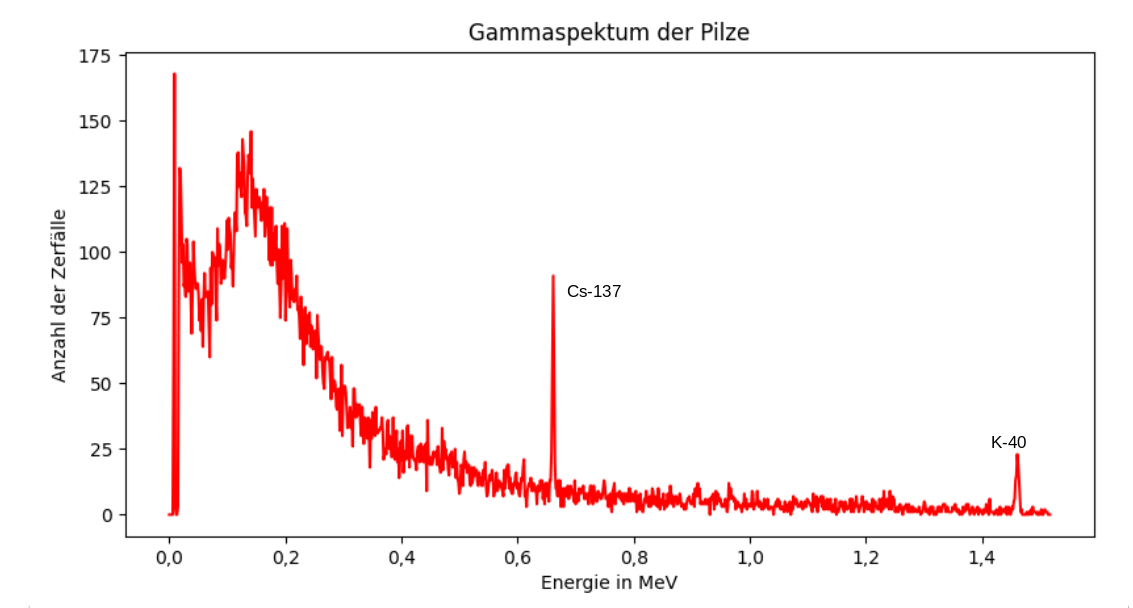
\includegraphics[width = 12cm]{Bilder/Auswertung/Pilze.png}
    \caption{Deutlich sichtbar die Linie des Cs-137 Isotops}
\end{figure}

Diese liegt bei $E_{Linie} =0,6615 \mathrm{MeV}$. Dabei ist diese identisch mit der Spektrallinie des Cs-137 Isotops, welches wir für die 
Energieeichung verwendet haben (siehe Tabelle \ref{Eichung}). Dort lag die Linie bei $E_{Cs-137} = 0,6616 \mathrm{MeV}$.\\
Der minimale Unterschied der beiden Werte lässt sich durch den 
Quantisierungsfehler bei Übertragen des kontinuierlichen Spektrums auf diskrete Werte erklären und einer möglicherweise leichten unlinearität des Vierkanalanalysators.
Im gesamten kann man sagen, dass die Pilze mit nahezu an Sicherheit grenzender Wahrscheinlichkeit Cs-137 enthalten.